\newpage
\chapter{Реализация}\label{ch:chapter_2}

\section{Middleware For Collaboration Implementation}

There is a lot of ways to achieve network communication between applications
starting from assembling raw TCP/IP datagrams up to using object-oriented
libraries for specific application-level protocols. We stated a list of
requirements to choose an appropriate middleware technology. These requirements
were collected from the three sources: our view of collaboration, restrictions
imposed by the target platforms and a preliminary architecture of the
application.

According to our view of collaboration (see section \ref{})
we have a server and several clients. For the sake of simplicity we assume that a server is allowed to be created anytime. Clients connect to server and modify
the shared mind map. Every change of the map is propagated via the server, which
notifies all the clients about it. For robust communicating all the participants
must always have the exact copy of the mind map.

HiveMind is now targeted at both mobile devices and PCs. Each platform gives us
unique advantages. PC users usually have wide broadband Internet
connection. Mobile devices can gain Internet access almost anytime and
anywhere. Due to the lack of IPv4 addresses mobile operators often assign
private IP addresses to mobile devices that makes them unreachable from the
Internet. Data transmission via wireless media sometimes causes unreasonable
delays for several seconds or more. PC users can use NAT or complex firewall
software that blocks incoming connections. It may be even worse: in corporate
environments users are often limited to HTTP proxy as the only source of the
Internet connection.

Summarizing all these challenges we get the following list of requirements for
middleware technology.
\begin{itemize}
\item Communication is based on the client-server model.
\item Server supports for subscription.
\item Users may have a slow unreliable connection to the Internet through the
  NAT gateway.
\item There must be no additional effort to set up the server.
\item Middleware must be supported by a Python library.
\end{itemize}

%This is not full list of requirements. It can be filled up with these
%statements. They cover additional functionality.
%\begin{itemize}
%\item Technology should support transient or backup server to reinforce
%communication between nodes.
%\item Messages may be encrypted to ensure the privacy of shared map.
%\item Technology should support instant messaging system.
%\end{itemize}

We compared several alternative technologies and chose the XMPP protocol as it
allows us to avoid almost all concerns about implementation of client-server
communication.

XMPP protocol can be considered at the several levels of abstraction. At the low
level there is a XMPP client application that connects to the XMPP server and
exchanges messages with it. Connection can be established in many ways, even on
top of HTTP protocol. At the higher level of abstraction the client gains access
to the whole network, where every node has unique identifier (JID) and no
additional effort required to exchange information between them. The client
creates a message addressed to another client and sends it to the server, which
handles all the routine to deliver the message.

Another great feature of XMPP is protocol extensions (XEP). 
XMPP is an open protocol and anyone may create a custom high-level protocol on
top of it. XMPP Standards Foundation manages the process of creation and
maintenance of such protocols. There is XEP-0060 Publish-Subscribe extension
\cite{xep-0060}. It defines how to implement publish/subscribe services on top
of XMPP. Any member of the network can create pub/sub service. XMPP protocol
with Publish-Subscribe extension fits the best into our requirements and that is
why it is our choice for middleware technology.

XMPP protocol is XML-based, and it may seem that using this protocol would
require broadband Internet connection, but it is not so. Intercommunication
between XMPP client and server may be compressed when XEP-0138 (Stream
Compression extension) enabled.

Nowadays a lot of public XMPP servers (e.g. jabber.ru) support for chatting. And
it is well-known that participating in chats is successful even when using
mobile phones without neccessity of broadband Internet connection. From the
technical point of view collaborative mind mapping looks very similar to chat
participation and expected traffic volume looks comparable. The only exception
relates to the device being a server, which may require broader connection to
communicate with lots of clients. This question will be addressed during the
further development of the HiveMind network subsystem.

The next task was to find a pure Python XMPP library that supports XEP-0060
extension. There are eight Python libraries listed at the XMPP Foundation
Website \cite{xmpp}. Some of them are discontinued (jabber.py), some are
targeted at newer (2.6, 3.x) Python releases which are unavailable on Maemo
platform (pyxmpp), the others represent research projects and are not suitable
for production environment (SleekXMPP). Twisted is the only XMPP library
available in Maemo repository.

Twisted framework does not include support for Publish-Subscribe extension but
there is an external full-featured implementation named wokkel.
It is not present in maemo repository. To base our application on top of that 
library, we need to create and maintain package for maemo platform. This is
additional effort we need to make to enable support for mobile devices.

XMPP protocol was created as an instant messaging protocol. It is convenient to
exchange human-readable messages in human-readable format. For the sake of 
interoperability it uses XML-based structures for message formatting. 

\section{Protocol For Collaboration}

% really awful beginning
 The development of any complex protocol and it implementation is a
 labour-consuming process. Our development team had no previous experience in
 such field and thus we decided to use iterative approach. At the first iteration
 protocol for the team work should be as simple as possible. Thereby allow us to
 develop network architecture and to test selected libraries.

 % data structure
 Publish-Subscribe extension requires to share information in the form of nodes
 and items. Node-item system can be compared with file system, where nodes
 represent directories and items represent files. Each item may have unique
 identifier. Subscriber can retrieve items from service either by name or get a
 number of last published items. Items should contain a valid XML data.

 HiveMind has undo/redo capabilities as any good document editor does. Now they
 are implemented on top of QUndoStack. When user makes a change to the mind map
 QUndoCommand is created and pushed into the stack. This allows the user to
 travel through the history of modifications. We decided to use undo/redo stack
 to model data structures of the protocol. All mind map data can be placed
 inside a single node. First item must contain XML-serialized mind map. All other
 items hold small changesets, witch users make to shared map. These modifications
 are the XML-serialized versions of QUndoCommand.

 \begin{figure}[!h]
 \centering
 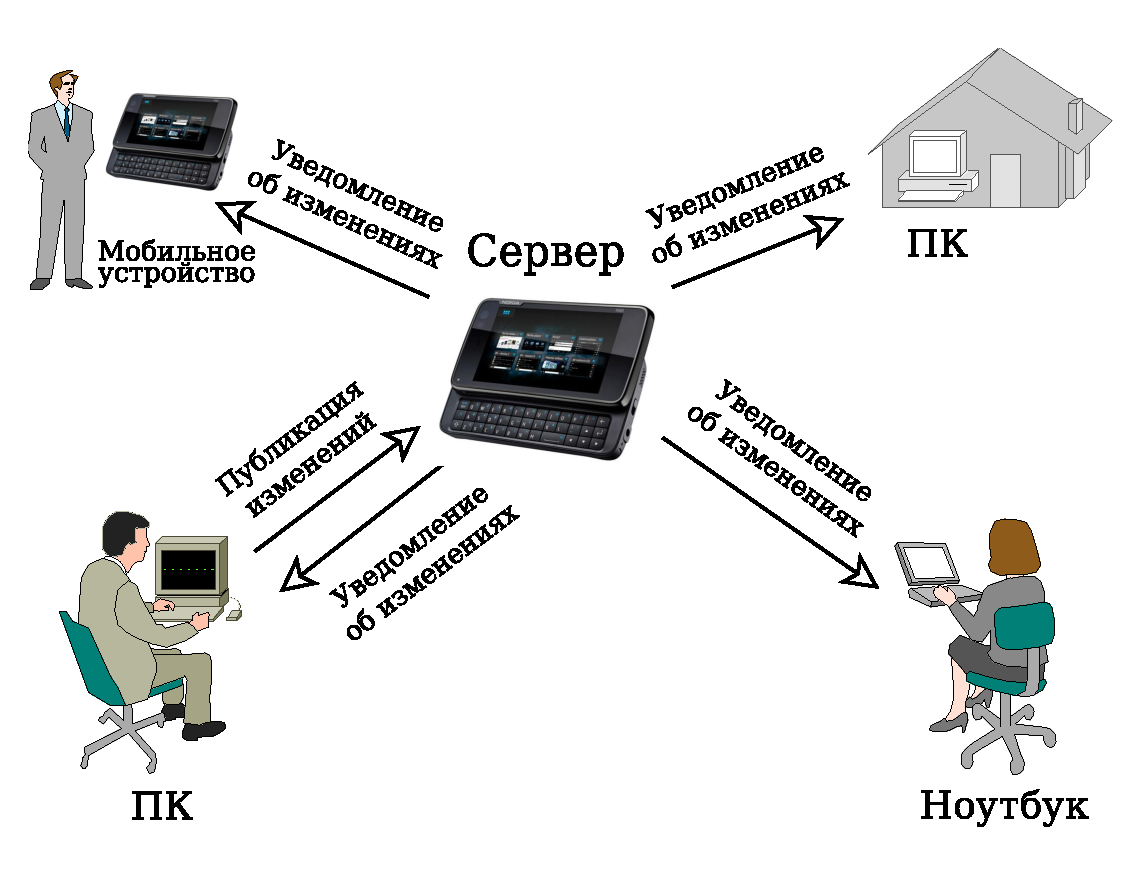
\includegraphics[width=\linewidth]{users_collaboration_example.pdf}
 \caption{Propagation of mind map changeset}
 \label{users_collaboration_example}
 \end{figure} 

 % notification propagation
 First item in the node is placed by the service in the moment of creation. Other
 items are published by participants of collaboration. Every new modification
 published in the node is retransmitted via update notifications to all
 subscribers and the service holder (see fig. \ref{users_collaboration_example}). 
 Service may reject the changeset if there are some defects (e.g. user wants to 
 update mind map node when it was already deleted by another user) and send error
 notification back to the subscriber.

 Protocol design proposes asynchronous propagation of modifications on the client
 side of publish/subscribe interaction. User changes to the mind map in the form
 of XML-serialized command are transmitted to the service and do not store in
 the local undo stack. Only changesets that were received as update notifications
 are added to the stack.

 Subscribers can retrieve all items stored in the node in any time. This
 way clients may synchronize contents of their local copy of mind map if
 transmitted changeset is rejected. Service does not need any additional effort
 to have up-to-date map because all notifications are local and can not be lost
 during transmission.

 To achieve this asynchronous process new element was added to the core of
 HiveMind --- NetworkController. It manages pub/sub protocol handlers. All
 QUndoCommands created as a result of mind map modifications are passed to the
 controller. If there is no network collaboration at the moment command will be
 sent back to MainWindowController and added to the local undo/redo stack.
 Otherwise command will be serialized and send to the service. Update
 notifications are deserialized into QUndoCommands and added to the undo/redo
 stack.

 The drawbacks of current collaboration protocol design and implementation
 include following statements. Client must wait for an update notification in
 order to see changes that he or she made to the shared mind map. Participants
 cannot use undo/redo commands.

 not 4 current document, may be next one
 There are brilliant examples on how to build iterative update shared space -
 Version Control Systems. Their main aim is almost the same as editing shared
 mind map: provide access to common space of source files. VCS can do all the 
 work here, but they do not provide any notification to all people involved in
 collaborative work. They use robust protocols, send only difference between
 committed versions, and do it really slow. \ldots

\section{Network Subsystem Architecture}

The XMPP protocol family is build out of two things: the core technology and the
XMPP Extension protocols (XEP). The core is responsible for the message exchange
between different parts of the system. Various extension protocols are built on
top of the core. The process of creation and maintenance of such protocols is
managed by XMPP Standards Foundation \cite{xmpp-standarts}.

The XMPP publish-subscribe extension \cite{xep-0060} uses the classic
``publish-subscribe'' or ``observer'' design pattern: a person or application
publishes information, and an event notification (with or without payload) is
broadcasted to all authorized subscribers. In general, the relationship between
the publisher and the subscriber is mediated by a service that receives
publication requests and broadcasts event notifications to subscribers.

Service may support several distinct entities available for subscription. These
entities are called ``nodes''. There are different notification lists for each
node hosted on the service. Publishers send data to the node and subscribers
receive event notifications from it. Nodes can also maintain history of events
and provide other services that supplement the pure pubsub model. Data send to
and from the node is called ``item''.

In terms of publish-subscribe extension the collaboration process can be
described as follows. A user creates a service and a single node for message
exchange. The other participants subscribe to the created node. When anyone
makes a change to the mind map it is sent to the service, which notifies all
participants about the change. The data is sent in the form of the item
payload. Having this principle scheme in mind, we began to form the teamwork
protocol and implement it in detail.

Each change to the mind map is atomic. All changes to the mind map are done with
the use of dialogs. When the edit operation is completed, QUndoCommand is
created and pushed into the command stack. For every change command type XML
serialization and deserialization functions are made.  The use of edit commands
causes the problem of sharing initial contents of the mind map. In order to
execute identical commands, all participants must have exact copies of the
initial mind map. In order to achieve this goal, the first item on the node must
contain XML-serialized mind map. All the other items, as discussed earlier, hold
serialized change commands.  When a participant subscribes to the node he/she
receives all the data stored in the node.

% notification propagation

\begin{figure}
\centering
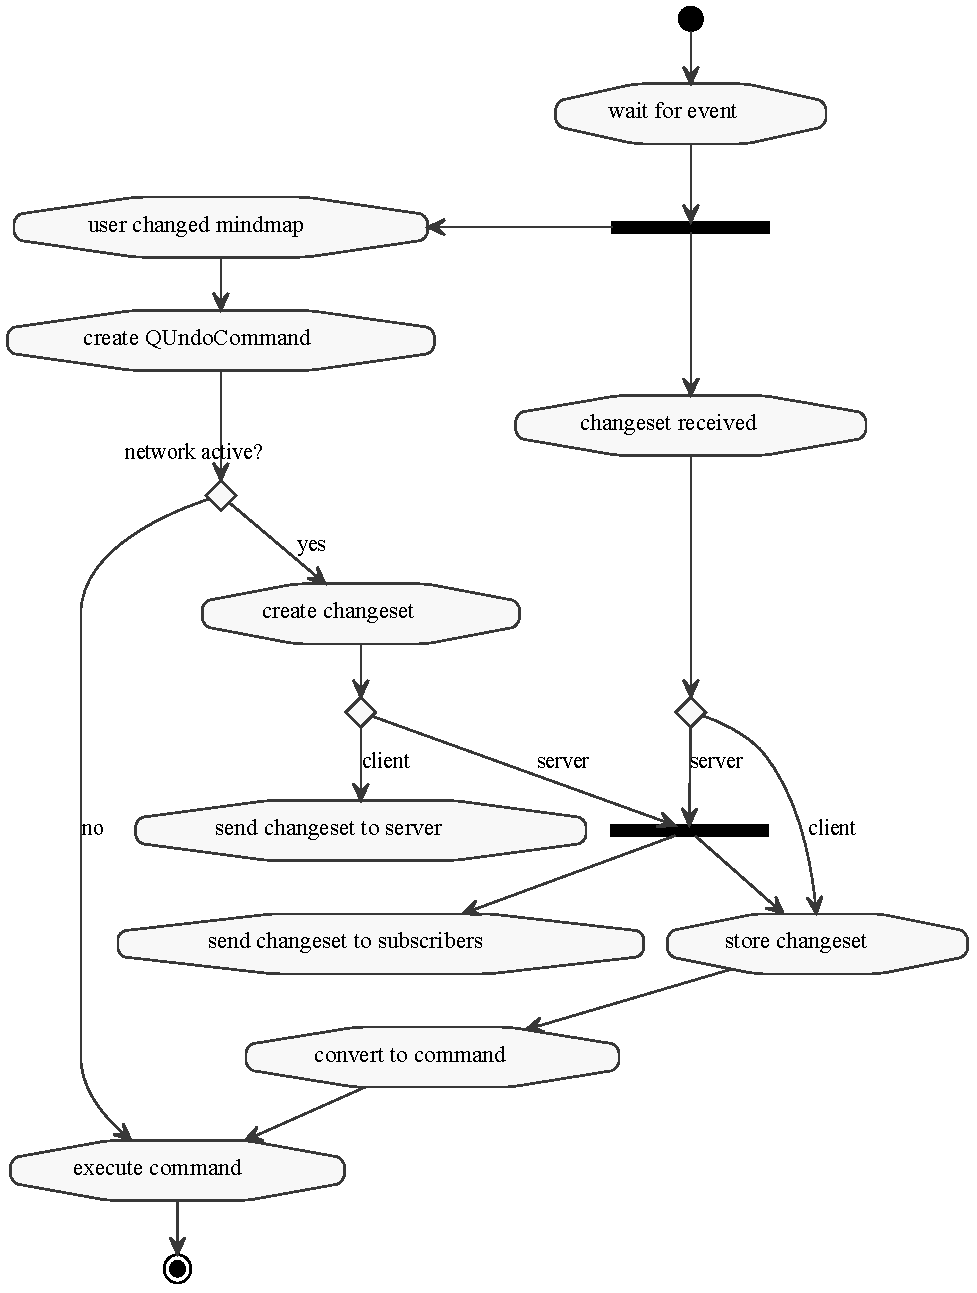
\includegraphics[width=0.8\linewidth]{changeset-propagation.pdf}
\caption{Changeset propagation}
\label{Changeset propagation}
\end{figure}

Each modification published in the node is recorded as a ``changeset''. The
changeset holds information about type of change, time it was formed, and the
author of the change (see fig.~\ref{Changeset propagation}). Service may reject
the changeset if it is irrelevant (e.g. user tries to update mind map node when
it was already deleted by another user) and send error notification back to the
subscriber.

Protocol design proposes asynchronous propagation of modifications on the client
side of publish/subscribe interaction. Modifications to the mind map are
transmitted to the service in the form of XML-serialized commands and are not
stored in the local undo stack. The only changesets received via update
notifications are added to the stack. So, the subscriber must wait for the
correct notification from the service in order to see changes that he or she has
made to the mind map.

The subscribers can retrieve all items stored in the node anytime. This
capability is used to synchronize contents of their local copy of the mind map
if transmitted changeset is rejected. Service does not need any additional
effort to have up-to-date map because all notifications are local and cannot be
lost during transmission.

To implement this asynchronous process, we introduced a new element to HiveMind
core --- NetworkController. It manages publish-subscribe protocol handlers. All
QUndoCommands, created as a result of mind map modifications, are passed to the
controller. If there is no network collaboration at the moment, the command will
be added to the local undo/redo stack. Otherwise, command will be serialized and
sent to the service. Update notifications are deserialized into QUndoCommands
and added to the undo/redo stack.


\section{Implementation of Network Subsystem}

Network subsystem of HiveMind is implemented on top of Twisted \cite{twisted} and
Wokkel \cite{wokkel}. Twisted is a framework for writing asynchronous,
event-driven network applications in Python. It has additional support for many
GUI frameworks like Qt, GTK, Tk, and others.

Wokkel library is a pack of enhancements for Twisted. Particularly, Wokkel
provides a mechanism for easier implementation of XMPP Enhancement Protocols
(XEP). It supports for Service Discovery (XEP-0030), Publish-Subscribe
(XEP-0060) and other XEPs. Implementation of XEP-0060 does not contain business
logic. It means that Wokkel responds for receiving and generating XMPP requests
according to XEP-0060 specification. Wokkel reacts on external pub/sub events
and invokes corresponding methods.

XEP-0060 is very large and complicated. Implementation of all features,
necessary for HiveMind, would take lots of time. Idavoll library is built on top
of Wokkel and provides implementations of many XEP-0060 features such as
``Subscribing'', ``Publishing'', ``Persistent items'', ``Node creation'' and
etc.

\begin{figure}
\begin{minipage}[t]{0.65\linewidth}
\center{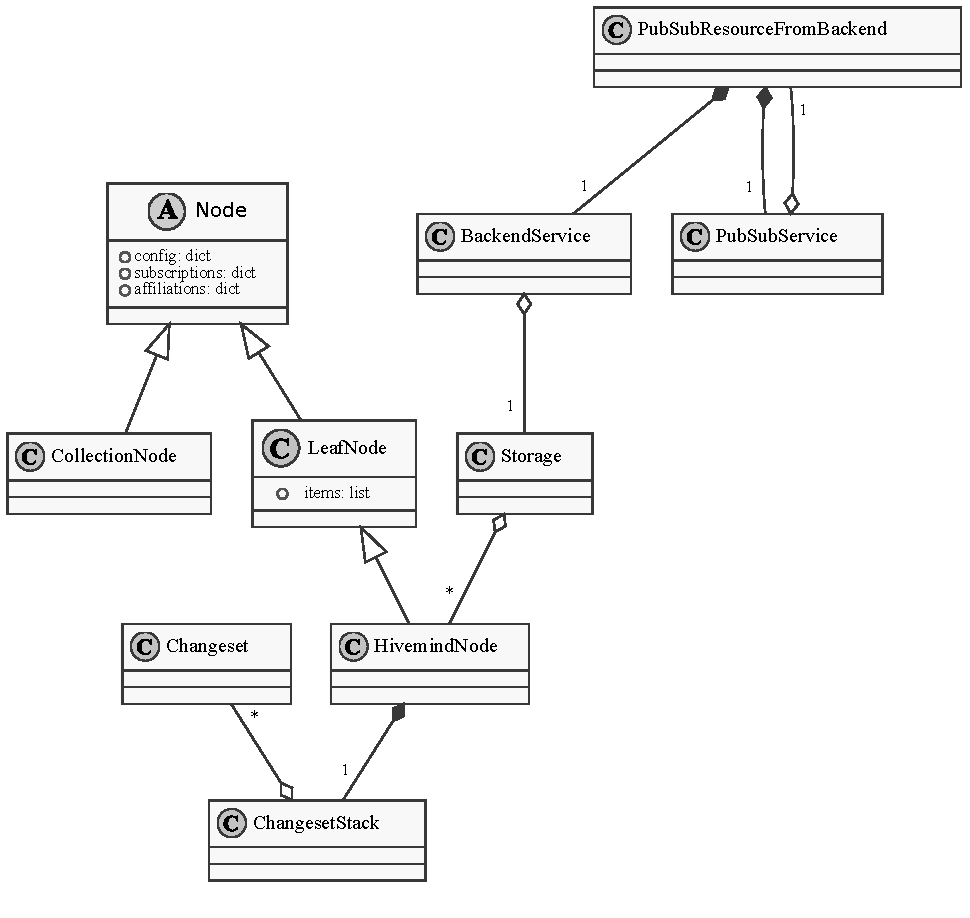
\includegraphics[width=\linewidth]{idavoll-classes.pdf}}
  \caption{Hierachy of network classes}
  \label{Network classes}
\end{minipage}
\hfill
\begin{minipage}[t]{0.35\linewidth}
\center{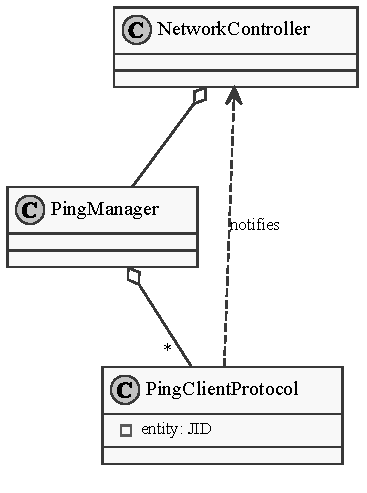
\includegraphics[scale=0.8]{ping-manager.pdf}}
  \caption{PingManager interaction}
  \label{Ping manager}
\end{minipage}
\end{figure}

Idavoll has many classes needed to implement XEP-0060 specification (see
fig.~\ref{Network classes}). Node class represents a XEP-0060 node. There are
two node types: Leaf and Collection. A leaf node contains a published item,
whereas a collection node contains other nodes.

HivemindNode class inherits LeafNode, but stores the published items in
ChangesetStack instead of a simple list. Using of ChangesetStack allows to check
integrity and correctness of data. Storage class responds for managing all nodes
on the service. BackendService is an implementation of XEP-0060 business logic.
PubSubServiceFromBackend inherits Wokkel's PubSubService class. It invokes
methods for handling corresponding XMPP requests and delegates action performing
to BackendService class.

Mobile devices often have unstable internet connection, so the user have to be
notified when XMPP session is lost. We check connection using XEP-0199 (XMPP
Ping) \cite{ping-xep-0199}. PingClientProtocol class sends ping to the XMPP
server and waits for reply. If there is a certain number of failed pings, the
connection is considered as lost.

The similar mechanism is used for checking participation status of a person. On
the service each participant has his/her own instance of PingClientProtocol. Ping
handler on the client side replies only to the service which it is connected
to. We implemented PingManager class to manage multiple instances of
PingClientProtocol (see fig.~\ref{Ping manager}).  It creates/deletes instances
and starts/stops ping to the certain entity. PingClientProtocol class is
responsible for notifying NetworkController about participant status, which is
shown to the service owner (see fig.~\ref{Permissions dialog}).

\begin{figure}[b] \centering
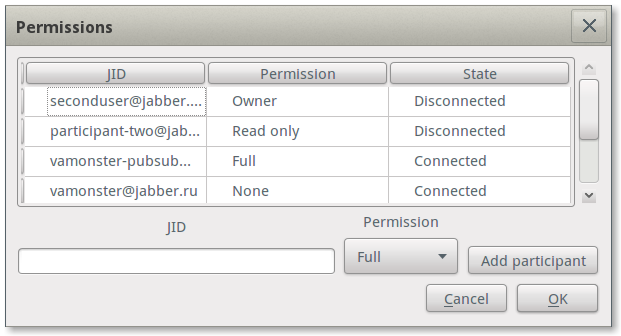
\includegraphics[width=0.5\linewidth]{permissions_dialog.png}
  \caption{Permissions dialog}
  \label{Permissions dialog}
\end{figure}

\section{Access Control System}
\label{Access control system}

By default, all participants of teamwork have equal permissions to contribute to
the mind map. It is quite convenient for brainstorming-like activities when the
purpose of the collaboration is to generate some materials or to find a solution
for a long-standing problem. This kind of behavior looks unsuitable for other
use cases. Sometimes it is useful to restrict access for particular users in
order to prevent accidental interference of teamwork. To take such scenarios
into account we introduced access control system to HiveMind.

XEP-0060 provides a feature, named Access Model, which can be associated with
authentication system. The user, who creates the mind map, can set trust level
for all new participants i.e. control who can participate in collaboration.
There are four access models implemented in HiveMind:
\begin{itemize}
\item ``Open'' --- any person may join collaboration;
\item ``Roster'' --- only contacts from the owner’s roster may join;
\item ``Authorize'' --- the owner choose who may join on the fly. When a new
  person is connected, the owner gets a participation request from the person;
\item ``Whitelist'' --- a person may join only if he/she is in the owner’s
  whitelist.
\end{itemize}

``Affiliations'' is the next feature, defined in XEP-0060, being a part of
HiveMind access control system. This feature provides authorization capabilities
to XEP-0060. After the person joined collaboration, he/she has a role, which
determines a set of allowed actions. There are four roles implemented in
HiveMind:
\begin{itemize}
\item ``Outcast'' --- person not allowed to join collaboration i.e. in terms of
  IM he/she is banned;
\item ``Member'' --- person allowed to receive items;
\item ``Publisher'' --- person allowed to publish and receive items;
\item ``Owner'' --- similar to the Publisher, but allowed to configure
  collaboration behaviour.
\end{itemize}
Service owner can edit role of desired person at any time with the use of
permissions dialog (fig.~\ref{Permissions dialog}).

XEP-0060 has features that makes access control even more flexible. In some
cases it might be useful to temporarily assign publisher role to all
participants. HiveMind has implementation of XEP-0060 feature named Publish
Model. It determines two cases of who is allowed to make changes to the
mindmap. In the first case it is a person whose affiliation is publisher, and in
the second case any participant is allowed to post changes.

Impelementation of access control system helps us to discover new use cases of
HiveMind. Presentation using HiveMind is one of such use cases. First of all,
lecturer can control who may join the presentation. Secondly, there are can be
more than one lecturer. Presentations using HiveMind distinguish from
collaborative editing: lecturer's current node and fold/unfold events must be
propagated through the network. This ensured that participants can track the
presentation movement.
 
Authorization system can be extended to greatly improve presentation
support. For example, lecturer may want to receive questions. Participants
can add nodes containing a questions or suggestions to lecturer mindmap.
Authorization system controls interaction between lecturer and participants e.g.
participant is able to modify only his own nodes and not able to modify nodes
created by lecturer or other participants.
